\chapter{Resultados}

Dependiendo del trabajo realizado, los resultados presentados pueden consistir de programas, paquetes, algoritmos, o estadígrafos, entre otros.

\section{Diagramas}
Los diagramas deben ser realizados en formato PDF e incluidos en el documento. Deben ser referenciados mediante referencias cruzadas. Por ejemplo:

\textbf{foRgotten} hace uso de paquetes externos para su correcto funcionamiento. El paquete \texttt{wBoot} \parencite{wBoot} interactúa con las funciones \texttt{directEffects()} y \texttt{bootMargin()} para aplicar \emph{bootstrap} con la prueba Z. El paquete \texttt{ggplot2} \parencite{ggplot2} permite generar el plano \emph{Dependence-Influence} en \texttt{bootMargin()}. El paquete \texttt{igraph} \parencite{igraph_article} permite aplicar la centralidad \emph{betweenness} en la función \texttt{centrality()}. El paquete \texttt{poweRlaw} \parencite{gillespie2014fitting} permite implementar el método de \textcite{clauset2009power} para determinar si la distribución de las centralidades es una distribución de potencia. El paquete \texttt{boot} \parencite{BootstrapMethods} permite aplicar \emph{bootstrap} en las funciones \texttt{centrality()} y \texttt{FE()}. Por ultimo, el paquete \texttt{Rcpp} permite acelerar el procesamiento de datos de la función \texttt{FE()} al escribir algunas funciones internas en código C++. La interacción con cada una de las funciones con los paquetes externos ya descritos se aprecia en la figura \ref{figure: diagrama-1}.


\begin{figure}[H]
  \centering
  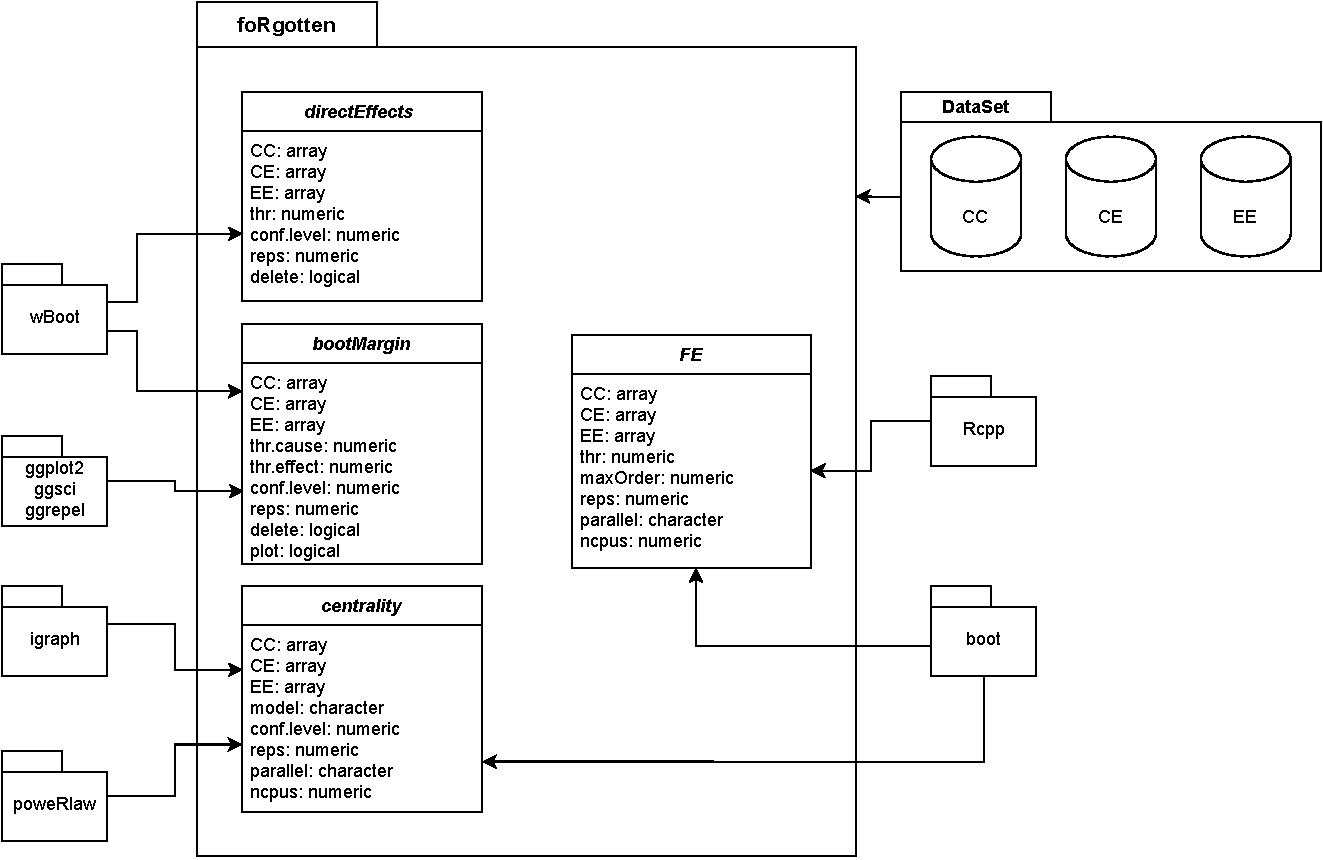
\includegraphics[width=\textwidth]{files/ESTRUCTURApaquete.pdf}
  \caption{Representación gráfica del paquete \textbf{foRgotten}}
  \label{figure: diagrama-1}
\end{figure}

\section{Datos}

En el caso de utilización de datos para el trabajo de título, debe darse cuenta de la fuente y estructura de los mismos. Por ejemplo:

Ilustramos el uso del paquete \textbf{foRgotten} con los datos de políticas publicas sobre contaminación atmosférica de l a comuna de Valdivia, Chile (PDA, Plan de Descontaminación Atmosférica para la comuna de Valdivia, en la
Resolución Exenta N° 839, de 24 de Agosto de 2015).  El conjunto de datos previamente procesado por \textcite{manna2018application} considera incentivos para fomentar el cambio de comportamiento en la política publica sobre descontaminación atmosférica. Se consideran dieciséis incentivos y cuatro comportamientos los cuales se describen en los cuadros \ref{tab: incentivos} y \ref{tab: comportamientos}.


\begin{table}[H]
\centering
\caption{Incentivos }
\label{tab: incentivos}
\resizebox{\textwidth}{!}{%
\begin{tabular}{@{}ll@{}}
\toprule
Código & Incentivos                         \\ \midrule
I1     & Prohibición                        \\
I2     & Norma (reglamento)                 \\
I3  & Subvención para dispositivos de calefacción para los servicios públicos \\
I4  & Subvención para dispositivos de calefacción para los hogares                      \\
I5     & Registro (inventario, información) \\
I6     & Leña seca                          \\
I7     & Inspección y auditoría             \\
I8     & Mejora y producción                \\
I9     & Subvención para leña               \\
I10 & Subvención para el aislamiento térmico de viviendas                               \\
I11    & Educación                          \\
I12    & Subvención para calderas           \\
I13    & I+D, investigación y desarrollo    \\
I14    & Subvención para transporte         \\
I15 & Sistema de evaluación de impacto ambiental                                        \\
I16    & Mitigación                         \\ \bottomrule
\end{tabular}%
}
\end{table}

\begin{table}[H]
\centering
\caption{Comportamientos}
\label{tab: comportamientos}
\resizebox{\textwidth}{!}{%
\begin{tabular}{@{}ll@{}}
\toprule
Código & Comportamientos                                     \\ \midrule
B1     & La gente mejora el aislamiento térmico de las casas \\
B2 & Las personas mejoran la eficiencia de los equipos de combustión de leña y sus componentes \\
B3 & La gente mejora la calidad de la leña y la disponibilidad de otros combustibles           \\
B4     & Educación y concienciación en la comunidad          \\ \bottomrule
\end{tabular}%
}
\end{table}

\section{Plataforma informática de trabajo y parámetros de simulación}
Siempre que se debe describer la plataforma informática de trabajo (tanto hardware como software) utilizada en el trabajo de título. Esto puede hacerse en un cuadro o directamente en el texto. Igualmente con los parámetros de simulación cuando deba hacerse uso de ellos. Por ejemplo:

\begin{table}
    \centering
    \caption{Especificaciones de hardware y software}
    \resizebox{\columnwidth}{!} {
    \begin{tabular}{|c|c|}
        \hline
        \textbf{Hardware}&
        \textbf{Especificación}\\
        \hline
        \multicolumn{2}{|c|}{Especificaciones de GPU}\\
        \hline
        Modelo de GPU & Geforce RTX2070 SUPER \\
        Cuda Cores & 2560\\
        SM & 40\\
        Base Clock(MHz) & 1605\\
        Memoria & 8GB DDR6 \\
        Velocidad de Memoria & 14Gbps \\
        \hline
        \multicolumn{2}{|c|}{Especificaciones Memoria RAM}\\
        \hline
        Capacidad &  16GB \\
        Velocidad base(MHz) & 3000 \\
        Tipo de Memoria & DDR4 \\
        \hline
        \multicolumn{2}{|c|}{Especificaciones de CPU}\\
        \hline
        Modelo de CPU & Ryzen 9 \\
        Cantidad de núcleos & 12\\
        Cantidad de hilos & 24\\
        Base Clock(GHz) & 3.8 \\
        \hline
        \textbf{Software}&
        \textbf{Especificación}\\
        \hline
        Sistema Operativo & Arch Linux 5.7.7-zen1-1-zen x86\_64 GNU\/Linux\\
        Cuda SDK & 10.2 \\
        \hline
    \end{tabular}
    }
    \label{tab:computador}
\end{table}


El algoritmo es ejecutado en un computador descrito en el Cuadro \ref{tab:computador} utilizando como parámetros los presentados en el Cuadro \ref{tab:parametros_recocido_simulado}. De cada combinación bloques-hilos se realizaron 30 réplicas (el número máximo de hilos considerado fue de 85 pues es el número de escuelas de Temuco).

\begin{table}
    \centering
    \caption{Valores de parámetros para todas las instancias del recocido simulado paralelo}\label{tab:parametros_recocido_simulado}
    \begin{tabular}{|c|c|c|c|}
        \hline
        \textbf{Configuración} & \textbf{Valores}  & \textbf{Configuración} & \textbf{Valores}\\
        \hline
        $T_{0}$ & 100000 & $\alpha$ & 0.98\\
        $T_{\min}$ & 0.00000009 & $\gamma_1$ & 0.214 \\
        $n$ & 29853 & $\gamma_2$ & 0.429 \\
        $m$ & 85  & $\gamma_3$ & 0.357\\
        $l_{1}$ & $m$ &  $b$ & (32,64,128,256)\\ 
        $l_{2}$ & $2\cdot m$ & $h$ & (1,32,64,85) \\
        \hline
    \end{tabular}
\end{table}

\section{Resultados de salida de programas}
Los resultados de salida del programa creado o utilizado deberan presentarse de manera tabular y ser referenciados con referencias cruzadas. Evitar hacer capturas de pantalla salvo que sea necesario para explicar un aspecto de la interfaz. Por ejemplo:

Veamos los primeros 10 elementos de \texttt{result\$DirectEffects}:
\DefineVerbatimEnvironment{example}{Verbatim}{fontsize={\fontsize{11.5pt}{11.6pt}\selectfont}}
\begin{example}
   From  To  Mean   UCI p.value
1    I1  I2 0.525 0.645   0.615
2    I1  I3 0.450 0.590   0.256
3    I1  I4 0.525 0.665   0.616
4    I1  I5 0.465 0.645   0.371
5    I1  I6 0.645 0.790   0.872
6    I1  I7 0.815 0.870   1.000
7    I1  I8 0.580 0.695   0.871
8    I1  I9 0.490 0.630   0.427
9    I1 I10 0.560 0.705   0.753
10   I1 I11 0.525 0.675   0.530
\end{example}

